\subsection{RAM}

\begin{figure}[H]
    \centering
    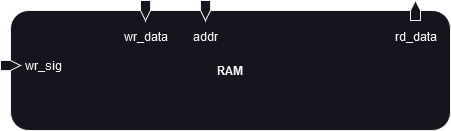
\includegraphics[width=0.75\textwidth]{../diagrams/rom_ram_reg/ram.png}
    \caption{RAM}
    \label{fig:ram}
\end{figure}

The RAM is the main memory of the CPU, it can be used to store and read values. In this project the RAM is also 1024 words long
and each word is 32 bits long.

Signals:
\begin{enumerate}[label={\textbullet}]
    \item Input: $addr$, This signal gives the address that needs to be read or written in the memory.
    \item Input: $wr\_sig$, This signal indicates if the given address need to be written or read
    \item Input: $wr\_data$, This signal gives the data that needs to be written in the memory.
    \item Output: $rd\_data$, This signal is representing the data that has been read from the RAM.
\end{enumerate}